\newpage
\subsection{考察}
まず,外皮アリ・ナシで尾びれの振り幅に差が出てしまった(図\ref{fig:kukkyoku})ことについて考察する.原因としては外皮に作った溝が胴体の屈曲を阻害し,本来胴体が屈曲するはずだった
位置まで動くことができなかったと考えられる(図\ref{fig:sogai}).実際に外皮を装着した状態で空中で振幅を測定した結果,プーリの回転角が$30\:^\circ$,
$45\:^\circ$,$60\:^\circ$のとき,尾ビレ振幅はそれぞれ$81\:^\circ$,$88\:^\circ$,$128\:^\circ$となった.本来の尾びれ振幅$81\:^\circ$,
$114\:^\circ$,$168\:^\circ$と比較すると約$40\:^\circ$差があることがわかった(表\ref{tb:amp}).ここで外皮なし・サーボ巻取り角30度の時81度,外皮あり・サーボ巻取り角45度の時
88度であり,比較的尾びれ振幅の条件としては近いことに着目する.このときの最高遊泳速度は外皮なしのとき186.7 mm/s,外皮ありのとき250.5 mm/sで外皮ありの条件の方が速い.これらのこと
から,外皮をつけることにより尾びれ振幅が小さくなってしまうというデメリットはあるものの,遊泳速度に関しては外皮をつけることによって向上すると言える.また尾びれ振幅が小さくならない
ような構造を実現することができれば,今回の結果よりもさらに優れた遊泳性能を示すと考えられる.

次に遊泳時に進行方向が傾いた(図\ref{fig:test_swim})ことについて考察する.昨年度卒業研究ではワイヤーの張力が左右に偏ることによって進行方向が傾いていたため,今回の実験では,ワイ
ヤーの張力が左右に偏るのを防ぐために,サーボモータの基準角度を変更することで左右の張力が偏らないようプログラムを組んでいた.しかし,基準角をプログラムで調整しても進行方向が少し傾い
\begin{table}[htbp]
    \centering
    \caption{サーボ巻き取り角と尾びれ振幅の関係}
    \label{tb:amp}
    \begin{tabular}{|c||c|c|}\hline
        サーボ巻き取り角[deg]&実験で使用した振幅[deg]&外皮装着時の振幅[deg]\\ \hline
        30&81&62\\ \hline
        45&114&88\\ \hline
        60&168&128\\ \hline
    \end{tabular}
\end{table}
\begin{figure}[hb]
    \centering
    \begin{tabular}{cc}
        \begin{minipage}[b]{0.4\linewidth}
            \centering
            \setPicture{gaihi_jama_nasi.png}
            \subcaption{外皮未装着時の胴体屈曲状態}
            \label{fig:jama_nasi}
        \end{minipage}
        \hspace{0.1\linewidth}
        \begin{minipage}[b]{0.4\linewidth}
            \centering
            \setPicture{gaihi_jama.png}
            \subcaption{外皮装着時の胴体屈曲状態}
            \label{fig:jama}
        \end{minipage}
    \end{tabular}
    \caption{外皮による屈曲の阻害}
    \label{fig:sogai}
\end{figure}
たり,遊泳実験をしている最中に今まで直進していた設定の時に進行方向が曲がってしまうことがあった.
原因として考えられることは2つある.1つ目は外皮を装着することによって胴体を屈曲させるためのトルクが増大し,それに伴って糸が伸びた,またはたるんでしまったということが考えられる.
2つ目はスタート時の姿勢が若干左右どちらかに傾いてしまったことにより,結果として左右に進行方向が傾いているように見えたと考えられる.
改善策として,糸の張力を一定にできる治具をロボットに取り付ける,もしくは使用するワイヤを現在使用しているワイヤよりも強度が高いものにするといったことがあげられる.

次に外皮ナシの状態の時に振幅の変化によってそこまで速度にそこまで大きな変化が無かった(図\ref{fig:amp})ことについて考察する.外皮無しで振幅$168\:^\circ$,周波数1.75 Hz時の遊泳時
の様子を見てみると(図\ref{fig:teikou})推進時に体が大きく屈曲してしまい,進行方向からの抵抗力を頭部と胴体部の一部で受けてしまっていることが分かる.これによっ
て本来その振幅で得られるはずだった推進力が低減し,遊泳速度が振幅によって変化しなかったと考えられる.
\begin{figure}[t]
    \centering
    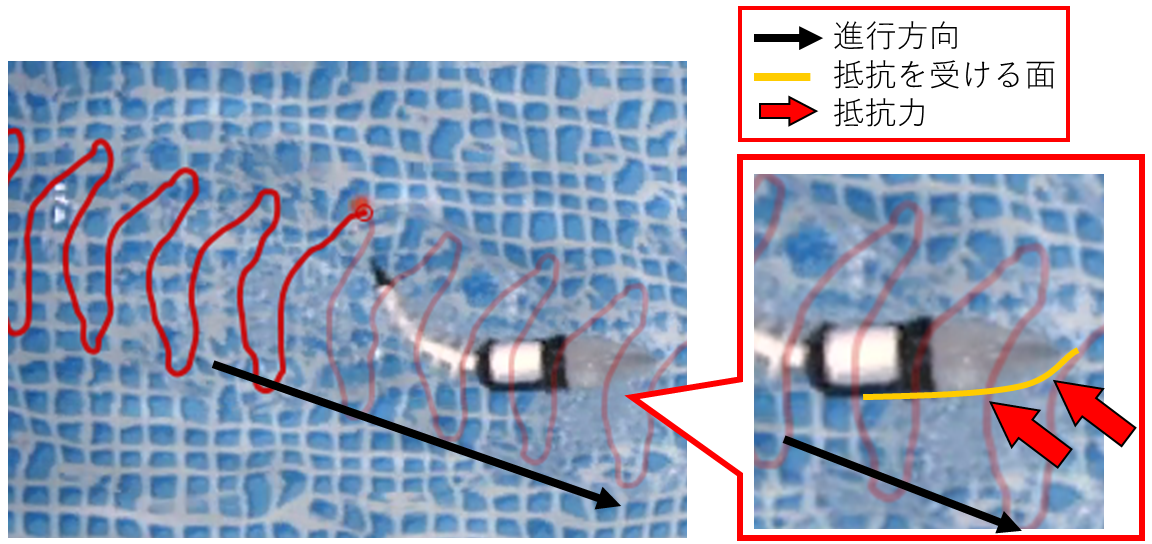
\includegraphics[width=0.9\linewidth]{chapters/picture/teikou.png}
    \caption{外皮未装着時に受ける抵抗}
    \label{fig:teikou}
\end{figure}
\begin{figure}[t]
    \centering
    \begin{tabular}{cc}
        \begin{minipage}[b]{0.45\linewidth}
            \centering
            \setPicture{compare_withoutskin.eps}
            \subcaption{外皮未装着時}
            \label{fig:without_matome}
        \end{minipage}
        \begin{minipage}[b]{0.45\linewidth}
            \centering
            \setPicture{compare_withskin.eps}
            \subcaption{外皮装着時}
            \label{fig:withskin_matome}
        \end{minipage}
    \end{tabular}
    \caption{外皮未装着時・装着時の結果をまとめたグラフ}
    \label{fig:matome}
\end{figure}
次に高周波数域において外皮が遊泳性能に与える影響について考察する.図\ref{fig:matome}に外皮有り・無しそれぞれの結果を1つのグラフにまとめたものを示す.グラフから低周波数域において
は外皮有り・無し両方において振幅による速度の変化はそれほど大きくは無かった.しかし,高周波数域を見てみると,外皮未装着時では振幅によってそこまで遊泳速度に差がない
のに対し,外皮装着時は振幅が大きくなるほど遊泳速度に差が出ていることが分かる.このことから高周波数域において柔軟外皮は遊泳性能に大きな影響を与えると考えられる.

\begin{figure}[t]
    \centering
    \setPicture{body.pdf}
    \caption{外皮の有無によるボディの違い}
    \label{fig:body}
\end{figure}

最後に外皮を装着することによってなぜ遊泳速度が向上したのかについて考察する.要因として考えられるのは外皮装着時と未装着時でボディが異なっていることである.外皮未装着時のボディは半流
線型のボディになっているのに対し,外皮装着時は流線型のボディになっている(図\ref{fig:body}).ここで流線型のボディはほかの形状に比べて物体の正面と背面の圧力差によって生じる圧力抵抗を低減することができ
る.したがって,ロボットのボディを流線型にすることによって水中で受ける抵抗力が減り,その分推進力が増大したと考えられる.
このことから,魚型ロボットに流線型のボディを備えることは遊泳性能の向上につながるといえる.

\subsection{今後の展望}
本研究では魚ロボットを用いて直進遊泳実験を行い,結果としてリンクの動きに追従できる柔軟外皮の開発に成功し,外皮によって遊泳速度が向上することも確かめられた.しかし,外皮によって胴体の屈曲が阻害され,
目的の振幅を得られないという問題があった.これについては外皮内部に作る溝の幅をあえてリンクより広めの幅で作製するか,サーボモータをより高トルクなものに変更することで解決できると考えられる.

ハード面では,本実験で用いた防水処理(IP67)を施されていたサーボモータが2回水没してしまったので,防水規格がIP68のモータに変更した方がよいと考える.また,本研究の実験結果から外皮装着時は周波数が高く,
振幅が大きいほど遊泳速度が向上するということがわかったが,この結果をもとにさらに速い速度で遊泳させようと周波数をだんだん高くすると,サーボモータが指令角度に到達する前に次の動作に移り,結果として振幅が
小さくなってしまう可能性がある.そこで今後はより多くの周波数で実験が可能になるようにサーボモータよりもより細かな制御が可能なブラシレスDCモータを使用し,遊泳速度の向上を図りたい.

また,遊泳形態について,本研究では直進性能しか検証できていないため,急旋回実験を行って旋回速度や旋回角度などの旋回性能を検証したい.
そして最終的には柔軟外皮の表面にウロコを配置し,対衝撃性能や遊泳性能への影響を検証し,魚らしい見た目を持った高機動性を有する魚ロボットの開発を目指す.